\documentclass[12pt, xcolor=table]{beamer}
\usepackage{graphicx}
\usepackage[ngerman]{babel}
\usepackage[utf8]{inputenc}
\usepackage{amsmath}
\usepackage{amssymb}
\usepackage{listings}
\usepackage{hyperref}
\usepackage{fancyvrb}
\usepackage{color}
\usepackage{verbatim}

\usepackage[percent]{overpic}
\usepackage[footnotesize, bf]{caption}
%Copyright 2008 by Adrian Böhmichen
%
% This file is free software: you can redistribute it and/or modify
% it under the terms of the GNU General Public License as published by
% the Free Software Foundation, either version 3 of the License, or
% (at your option) any later version.
%
% This file is distributed in the hope that it will be useful,
% but WITHOUT ANY WARRANTY; without even the implied warranty of
% MERCHANTABILITY or FITNESS FOR A PARTICULAR PURPOSE.  See the
% GNU General Public License for more details.
%
% You should have received a copy of the GNU General Public License
% along with this file.  If not, see <http://www.gnu.org/licenses/>.

%%%%%%%%%%%%%%%%%%%%%%%%%%%%%%%%%%%%%%%%%%%%%%%%%%%%%%%%%%%%%%%%%
%     Ubuntuusers Vorlage für ein LaTeX-Beamer Theme            %
%                                                               %
% Für das Korrekte funktionieren benötigt man einen header.png  %
% und ein logo.png Datei!                                       %
% Zusätzlich muss man folgende Pakete benutzten:                %
%   \usepackage{graphicx}                                       %
%   \usepackage[percent]{overpic}                               %
%                                                               %
% Danach muss nur noch am Anfang die Datei                      %
% mit \input{} eingebunden werden.                              %
%                                                               %
%%%%%%%%%%%%%%%%%%%%%%%%%%%%%%%%%%%%%%%%%%%%%%%%%%%%%%%%%%%%%%%%%

%weitere Farbe spezifizieren:
%Farben von dem Humantheme
%\definecolor{Orange}{RGB}{240,165,19}
\definecolor{Orange}{RGB}{5,215,242}
%\definecolor{Human-Base}{RGB}{129,102,71}
\definecolor{Human-Base}{RGB}{5,25,242}
%Farben aus dem Inyokatheme
%\definecolor{uuheader1}{RGB}{164,143,101}
\definecolor{uuheader1}{RGB}{5,25,242}
%\definecolor{uuheader2}{RGB}{129,106,59}
\definecolor{uuheader2}{RGB}{5,25,242}


%Theme festlegen für alle Templates die nicht selbstständig definiert werden:
\usepackage{beamerthemedefault}


%Definieren des Innertheme, zuständig für die Symbole bei Listen
\setbeamertemplate{sections/subsections in toc}[circle]
\setbeamertemplate{items}[circle]

\setbeamercolor{item}{fg=Human-Base}

%entfernen der Navigationsleiste
\beamertemplatenavigationsymbolsempty

%Logo definieren, man kann die Lage nicht verändern
%\logo{\includegraphics[scale=0.1]{logo.png}}


%Kopf- und Fußzeile definieren
%\setbeamertemplate{headline}
%{%
%\begin{overpic}[width=\paperwidth
% nächste Zeile dient zum anzeigen eines Rasters, für das paltzieren des ToC hilfreich
%,grid,tics=10
%]
%{header.png}%
%  \put(0,11){\insertsectionnavigationhorizontal{\paperwidth}{~}{~}}%
%  \end{overpic}
%}

\setbeamertemplate{footline}[text line]
{%
\begin{minipage}[b]{116mm}
\insertauthor \hfill%
%neue Navigationsleiste
 \insertframenumber ~/ \inserttotalframenumber\\[1ex]
\end{minipage}
}

% Farben festlegen ausserhalb des innertheme

%Allgemeine Angaben und Verbesserung vom default Theme
\setbeamercolor{structure}{fg=uuheader1}
\setbeamercolor{section in toc}{fg=Human-Base}
\setbeamercolor{subsection in toc}{parent=section in toc}
\setbeamercolor{framesubtitle}{fg=uuheader2}


%Farbe und Form der Blöcke definieren
\setbeamertemplate{blocks}[rounded]
%\setbeamercolor{block title}{fg=uuheader1,bg=Orange}
%\setbeamercolor{block title alerted}{use=alerted text,fg=black,bg=alerted text.fg!75!bg}
%\setbeamercolor{block title example}{use=example text,fg=black,bg=example text.fg!75!bg}

%\setbeamercolor{block body}{parent=normal text,use=block title,bg=block title.bg!25!bg}
%\setbeamercolor{block body alerted}{parent=normal text,use=block title alerted,bg=block title alerted.bg!25!bg}
%\setbeamercolor{block body example}{parent=normal text,use=block title example,bg=block title example.bg!25!bg}

%Für den Titleframe
\setbeamertemplate{title page}[default][rounded=true]
\setbeamercolor{title}{fg=uuheader2}
%,bg=Orange}


\makeatletter
\def\PY@reset{\let\PY@it=\relax \let\PY@bf=\relax%
    \let\PY@ul=\relax \let\PY@tc=\relax%
    \let\PY@bc=\relax \let\PY@ff=\relax}
\def\PY@tok#1{\csname PY@tok@#1\endcsname}
\def\PY@toks#1+{\ifx\relax#1\empty\else%
    \PY@tok{#1}\expandafter\PY@toks\fi}
\def\PY@do#1{\PY@bc{\PY@tc{\PY@ul{%
    \PY@it{\PY@bf{\PY@ff{#1}}}}}}}
\def\PY#1#2{\PY@reset\PY@toks#1+\relax+\PY@do{#2}}

\def\PY@tok@gd{\def\PY@tc##1{\textcolor[rgb]{0.63,0.00,0.00}{##1}}}
\def\PY@tok@gu{\let\PY@bf=\textbf\def\PY@tc##1{\textcolor[rgb]{0.50,0.00,0.50}{##1}}}
\def\PY@tok@gt{\def\PY@tc##1{\textcolor[rgb]{0.00,0.25,0.82}{##1}}}
\def\PY@tok@gs{\let\PY@bf=\textbf}
\def\PY@tok@gr{\def\PY@tc##1{\textcolor[rgb]{1.00,0.00,0.00}{##1}}}
\def\PY@tok@cm{\let\PY@it=\textit\def\PY@tc##1{\textcolor[rgb]{0.25,0.50,0.50}{##1}}}
\def\PY@tok@vg{\def\PY@tc##1{\textcolor[rgb]{0.10,0.09,0.49}{##1}}}
\def\PY@tok@m{\def\PY@tc##1{\textcolor[rgb]{0.40,0.40,0.40}{##1}}}
\def\PY@tok@mh{\def\PY@tc##1{\textcolor[rgb]{0.40,0.40,0.40}{##1}}}
\def\PY@tok@go{\def\PY@tc##1{\textcolor[rgb]{0.50,0.50,0.50}{##1}}}
\def\PY@tok@ge{\let\PY@it=\textit}
\def\PY@tok@vc{\def\PY@tc##1{\textcolor[rgb]{0.10,0.09,0.49}{##1}}}
\def\PY@tok@il{\def\PY@tc##1{\textcolor[rgb]{0.40,0.40,0.40}{##1}}}
\def\PY@tok@cs{\let\PY@it=\textit\def\PY@tc##1{\textcolor[rgb]{0.25,0.50,0.50}{##1}}}
\def\PY@tok@cp{\def\PY@tc##1{\textcolor[rgb]{0.74,0.48,0.00}{##1}}}
\def\PY@tok@gi{\def\PY@tc##1{\textcolor[rgb]{0.00,0.63,0.00}{##1}}}
\def\PY@tok@gh{\let\PY@bf=\textbf\def\PY@tc##1{\textcolor[rgb]{0.00,0.00,0.50}{##1}}}
\def\PY@tok@ni{\let\PY@bf=\textbf\def\PY@tc##1{\textcolor[rgb]{0.60,0.60,0.60}{##1}}}
\def\PY@tok@nl{\def\PY@tc##1{\textcolor[rgb]{0.63,0.63,0.00}{##1}}}
\def\PY@tok@nn{\let\PY@bf=\textbf\def\PY@tc##1{\textcolor[rgb]{0.00,0.00,1.00}{##1}}}
\def\PY@tok@no{\def\PY@tc##1{\textcolor[rgb]{0.53,0.00,0.00}{##1}}}
\def\PY@tok@na{\def\PY@tc##1{\textcolor[rgb]{0.49,0.56,0.16}{##1}}}
\def\PY@tok@nb{\def\PY@tc##1{\textcolor[rgb]{0.00,0.50,0.00}{##1}}}
\def\PY@tok@nc{\let\PY@bf=\textbf\def\PY@tc##1{\textcolor[rgb]{0.00,0.00,1.00}{##1}}}
\def\PY@tok@nd{\def\PY@tc##1{\textcolor[rgb]{0.67,0.13,1.00}{##1}}}
\def\PY@tok@ne{\let\PY@bf=\textbf\def\PY@tc##1{\textcolor[rgb]{0.82,0.25,0.23}{##1}}}
\def\PY@tok@nf{\def\PY@tc##1{\textcolor[rgb]{0.00,0.00,1.00}{##1}}}
\def\PY@tok@si{\let\PY@bf=\textbf\def\PY@tc##1{\textcolor[rgb]{0.73,0.40,0.53}{##1}}}
\def\PY@tok@s2{\def\PY@tc##1{\textcolor[rgb]{0.73,0.13,0.13}{##1}}}
\def\PY@tok@vi{\def\PY@tc##1{\textcolor[rgb]{0.10,0.09,0.49}{##1}}}
\def\PY@tok@nt{\let\PY@bf=\textbf\def\PY@tc##1{\textcolor[rgb]{0.00,0.50,0.00}{##1}}}
\def\PY@tok@nv{\def\PY@tc##1{\textcolor[rgb]{0.10,0.09,0.49}{##1}}}
\def\PY@tok@s1{\def\PY@tc##1{\textcolor[rgb]{0.73,0.13,0.13}{##1}}}
\def\PY@tok@sh{\def\PY@tc##1{\textcolor[rgb]{0.73,0.13,0.13}{##1}}}
\def\PY@tok@sc{\def\PY@tc##1{\textcolor[rgb]{0.73,0.13,0.13}{##1}}}
\def\PY@tok@sx{\def\PY@tc##1{\textcolor[rgb]{0.00,0.50,0.00}{##1}}}
\def\PY@tok@bp{\def\PY@tc##1{\textcolor[rgb]{0.00,0.50,0.00}{##1}}}
\def\PY@tok@c1{\let\PY@it=\textit\def\PY@tc##1{\textcolor[rgb]{0.25,0.50,0.50}{##1}}}
\def\PY@tok@kc{\let\PY@bf=\textbf\def\PY@tc##1{\textcolor[rgb]{0.00,0.50,0.00}{##1}}}
\def\PY@tok@c{\let\PY@it=\textit\def\PY@tc##1{\textcolor[rgb]{0.25,0.50,0.50}{##1}}}
\def\PY@tok@mf{\def\PY@tc##1{\textcolor[rgb]{0.40,0.40,0.40}{##1}}}
\def\PY@tok@err{\def\PY@bc##1{\fcolorbox[rgb]{1.00,0.00,0.00}{1,1,1}{##1}}}
\def\PY@tok@kd{\let\PY@bf=\textbf\def\PY@tc##1{\textcolor[rgb]{0.00,0.50,0.00}{##1}}}
\def\PY@tok@ss{\def\PY@tc##1{\textcolor[rgb]{0.10,0.09,0.49}{##1}}}
\def\PY@tok@sr{\def\PY@tc##1{\textcolor[rgb]{0.73,0.40,0.53}{##1}}}
\def\PY@tok@mo{\def\PY@tc##1{\textcolor[rgb]{0.40,0.40,0.40}{##1}}}
\def\PY@tok@kn{\let\PY@bf=\textbf\def\PY@tc##1{\textcolor[rgb]{0.00,0.50,0.00}{##1}}}
\def\PY@tok@mi{\def\PY@tc##1{\textcolor[rgb]{0.40,0.40,0.40}{##1}}}
\def\PY@tok@gp{\let\PY@bf=\textbf\def\PY@tc##1{\textcolor[rgb]{0.00,0.00,0.50}{##1}}}
\def\PY@tok@o{\def\PY@tc##1{\textcolor[rgb]{0.40,0.40,0.40}{##1}}}
\def\PY@tok@kr{\let\PY@bf=\textbf\def\PY@tc##1{\textcolor[rgb]{0.00,0.50,0.00}{##1}}}
\def\PY@tok@s{\def\PY@tc##1{\textcolor[rgb]{0.73,0.13,0.13}{##1}}}
\def\PY@tok@kp{\def\PY@tc##1{\textcolor[rgb]{0.00,0.50,0.00}{##1}}}
\def\PY@tok@w{\def\PY@tc##1{\textcolor[rgb]{0.73,0.73,0.73}{##1}}}
\def\PY@tok@kt{\def\PY@tc##1{\textcolor[rgb]{0.69,0.00,0.25}{##1}}}
\def\PY@tok@ow{\let\PY@bf=\textbf\def\PY@tc##1{\textcolor[rgb]{0.67,0.13,1.00}{##1}}}
\def\PY@tok@sb{\def\PY@tc##1{\textcolor[rgb]{0.73,0.13,0.13}{##1}}}
\def\PY@tok@k{\let\PY@bf=\textbf\def\PY@tc##1{\textcolor[rgb]{0.00,0.50,0.00}{##1}}}
\def\PY@tok@se{\let\PY@bf=\textbf\def\PY@tc##1{\textcolor[rgb]{0.73,0.40,0.13}{##1}}}
\def\PY@tok@sd{\let\PY@it=\textit\def\PY@tc##1{\textcolor[rgb]{0.73,0.13,0.13}{##1}}}

\def\PYZbs{\char`\\}
\def\PYZus{\char`\_}
\def\PYZob{\char`\{}
\def\PYZcb{\char`\}}
\def\PYZca{\char`\^}
\def\PYZsh{\char`\#}
\def\PYZpc{\char`\%}
\def\PYZdl{\char`\$}
\def\PYZti{\char`\~}
% for compatibility with earlier versions
\def\PYZat{@}
\def\PYZlb{[}
\def\PYZrb{]}
\makeatother

\renewcommand{\footnotesize}{\tiny}

\begin{document}
\title{Multilabel Classification}
\author{peterr und Lusy}
\date{\today}

\begin{frame}
    \titlepage
    \begin{block}{https://github.com/lusy/multilabel\_classification}
    \end{block}
\end{frame}

\begin{frame}
    \frametitle{Übersicht}
    \tableofcontents
\end{frame}

\section{Datensatz}
\begin{frame}
    \frametitle{Datensatz}
    \begin{itemize}
        \item mathematische Publikationen mit Titeln und Abstracts
        \item enthält  $1.1$ Mio. Dokumente
        \item jedes Dokument hat min. 1 Label
        \item $75.6 \%$ 1 Label, $24.3 \%$ 2 Label und ca. $0.1 \%$ mehr Labels
    %\item aus welchen Jahren sind die Publikationen
    \end{itemize}
    \begin{block}{Aufbau}
        \begin{itemize}
            \item[Doc:] [ID] [LABELS] [YEAR] [TITLE] [ABSTRACT]
        \end{itemize}
    \end{block}
\end{frame}

\section{Verteilung der Labels}
\begin{frame}
    \frametitle{Verteilung der Labels}
    \begin{center}
        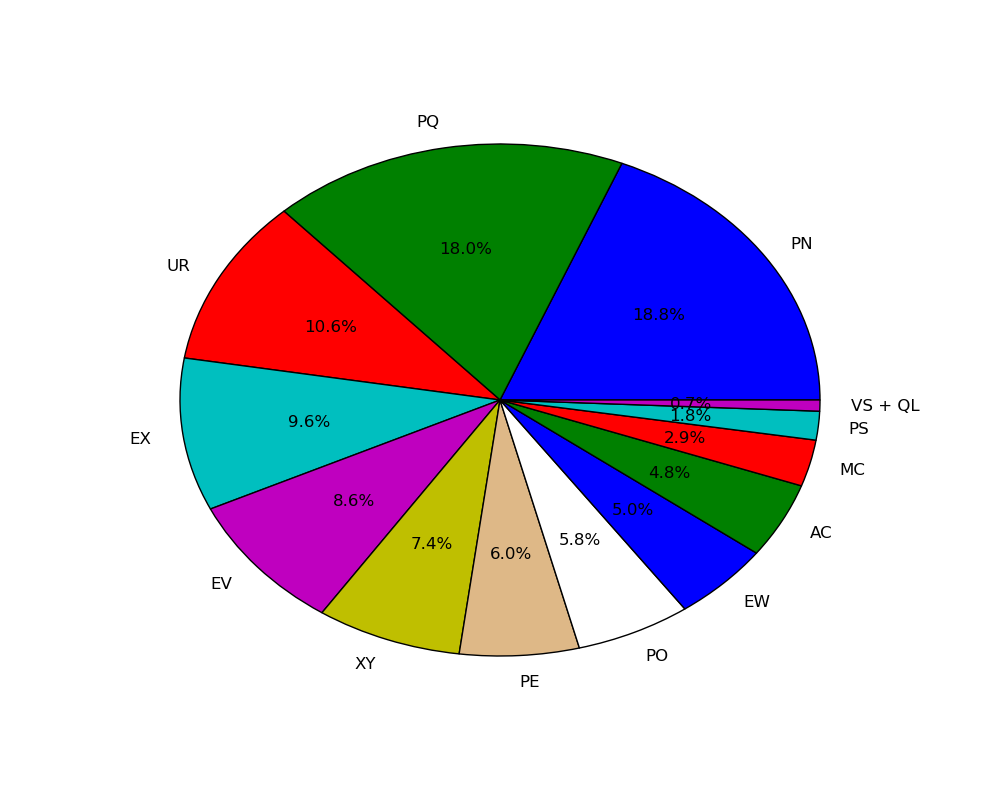
\includegraphics[scale=0.3]{figures/labels.png}
    \end{center}
    \begin{itemize}
        \item häufigstes Klasse: PN mit $266\, 198$ Dokumente
        \item seltenstes Klasse: QL mit $1448$ Dokumente
    \end{itemize}
\end{frame}

\section{Einführung}
\begin{frame}
    \frametitle{Einführung}
    \begin{block}{Zielsetzung}
        Verbesserung der Klassifizierung von Dokumenten mit Hilfe vonTopic Models
    \end{block}
    \begin{itemize}
        \item  Tools: python, bash, scikit-learn, liblinear, mallet
        \item  Vorverarbeitung: Stopwörter und Satzzeichen entfernen
        \item  Aufteilung in Test-($25 \%$) und Trainingsdatensatz($75 \%$)
        %\item  Corner stones?
        %\item  geschätzter/gemessener Aufwand (Speicher, Laufzeit)
        %\item  was beinhaltet sie überhaupt (Stratified Sampling, etc.)
    \end{itemize}
\end{frame}

\section{SVM} % (fold)
\label{sec:SVM}

% section SVM (end)
\begin{frame}
    \frametitle{SVM Klassifizierung}
    \begin{center}
    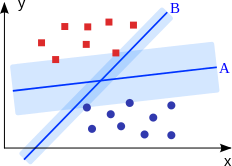
\includegraphics[scale=0.75]{figures/Svm_intro.png}
    \end{center}
    \begin{itemize}
        \item Margin maximieren
        \item verschiedene Kernel zur Trennung der Hyperebene
    \end{itemize}
\end{frame}

\section{Topic Models und LDA} % (fold)
\label{sec:LDA}

% section LDA (end)
\begin{frame}
    \frametitle{Topic Models und LDA}
    \begin{block}{Topic}
         Verteilung über Wörtern
    \end{block}
    \begin{block}{Dokument}
        diskrete Verteilung über Wörtern
        diskrete Verteilung über Topics
    \end{block}
    \begin{block}{LDA}
    \end{block}
\end{frame}
\section{Klassifikation} % (fold)
\label{sec:Klassifikation}

% section Klassifikation (end)
\begin{frame}
    \frametitle{Multiclass Classification}
    \begin{itemize}
        \item jeder Datensatz hat nur ein Label
        \item aber der gesamte Datensatz besitzt mehr als eine Klasse
        %\item Kenngrößen
        %\item Evaluationsgrößen: Recall, Precision, F1, micro and macro averaging
    \end{itemize}
    \begin{block}{Beispiel}
    \begin{center}
    \begin{table}
        \rowcolors[]{1}{blue!20}{blue!10}
        \begin{tabular}{ccc}
            \tiny\textbf{doc\_id} &\tiny \textbf{Label}  \\
            \hline
            \tiny 1 &\tiny A  \\
            \tiny 2 &\tiny B  \\
            \tiny 3 &\tiny B  \\
            \tiny 4 &\tiny C  \\
            \tiny 5 &\tiny A  \\
        \end{tabular}
         \caption*{Beispiel Multiclass mit Klassen A,B und C}
    \end{table}
    \end{center}
    \end{block}
\end{frame}

\begin{frame}
    \frametitle{Multilabel Classification}
    \begin{itemize}
        \item ein Label kann mehrere Klassen beinhalten
        \item One-Vs-One und One-vs-Rest Klassifizierer
        %\item Kenngrößen
        %\item Evaluationsgrößen: Recall, Precision, F1, micro and macro averaging
    \end{itemize}
    \begin{block}{Beispiel}
    \begin{center}
    \begin{table}
        \rowcolors[]{1}{blue!20}{blue!10}
        \begin{tabular}{ccc}
            \tiny\textbf{doc\_id} &\tiny \textbf{Label}  \\
            \hline
            \tiny 1 &\tiny A  \\
            \tiny 2 &\tiny B  \\
            \tiny 3 &\tiny B,A  \\
            \tiny 4 &\tiny C,A,B  \\
            \tiny 5 &\tiny A  \\
        \end{tabular}
         \caption*{Beispiel Multilabel mit Klassen A,B und C}
    \end{table}
    \end{center}
    \end{block}
\end{frame}

\begin{frame}
    \frametitle{Evaluation}
    \begin{itemize}
        \item Precision \[\frac{\#(\text{relevant items retrieved})}{\#(\text{retrieved items})}\]
        \item Reacall \[\frac{\#(\text{relevant items retrieved})}{\#(\text{relevant items})}\]
        \item F1-Measure \[F_1 = 2 \cdot \frac{\mathrm{precision} \cdot \mathrm{recall}}{\mathrm{precision} + \mathrm{recall}}\]
        \item micro average F1-Measure
        \item macro average F1-Measure
    \end{itemize}
\end{frame}

\section{Ergebnis auf Titeln} % (fold)
\label{sec:Ergebnis}

% section Ergebnis (end)
\begin{frame}
    \frametitle{Ergebnis mit Titel}
    \begin{center}
    \begin{table}
    \rowcolors[]{1}{blue!20}{blue!10}
    \begin{tabular}{c|cccc}
        \tiny\textbf{Klassen} &\tiny \textbf{unigram SVM} &\tiny \textbf{14 Topics SVM} & \tiny \textbf{50 Topics SVM} & \tiny \textbf{100 Topics SVM}\\
        \hline
        \tiny AC &\tiny 54\% &\tiny 15\% &\tiny 36 \% &\tiny 36 \%\\
        \tiny EV &\tiny 31 \% &\tiny 0.1\% &\tiny 4 \% &\tiny 7 \%\\
        \tiny EW &\tiny 22 \% &\tiny 0\% &\tiny 1 \% &\tiny 1.4 \%\\
        \tiny EX &\tiny 45 \% &\tiny 0.5\% &\tiny 20 \% &\tiny 22 \%\\
        \tiny MC &\tiny 46 \% &\tiny 0.0\% &\tiny 19 \% &\tiny 22 \%\\
        \tiny PE &\tiny 47 \% &\tiny 8\% &\tiny 26 \% &\tiny 26 \%\\
        \tiny PN &\tiny 46 \% &\tiny 31\% &\tiny 33 \% &\tiny 32 \%\\
        \tiny PO &\tiny 23 \% &\tiny 0\% &\tiny 0.4 \% &\tiny 1.9 \%\\
        \tiny PQ &\tiny 76 \% &\tiny 61\% &\tiny 64 \% &\tiny 64 \%\\
        \tiny PS &\tiny 44 \% &\tiny 0\% &\tiny 1 \% &\tiny 3 \%\\
        \tiny QL &\tiny 2 \% &\tiny 0\% &\tiny 0 \% &\tiny 0 \%\\
        \tiny UR &\tiny 65 \% &\tiny 28\% &\tiny 46 \% &\tiny 46 \%\\
        \tiny VS &\tiny 51 \% &\tiny 0\% &\tiny 0 \% &\tiny 0 \%\\
        \tiny XY &\tiny 62 \% &\tiny 34\% &\tiny 45 \% &\tiny 43 \%\\
    \end{tabular}
     \caption*{F1-Measures}
    \end{table}
    \end{center}
\end{frame}

%\begin{frame}
    %\frametitle{Multilabel Classification mit Dimensionsreduktion}
%\end{frame}


\section{Weiteres} % (fold)
\label{sec:Weiteres}

% section Weiteres (end)
\begin{frame}
    \frametitle{Probleme}
    \begin{itemize}
        \item unterschiedliche Klassengrößen
        \item Aufwand der Berechnungen(Speicher)
        \item Topicverteilung nicht sparse
    \end{itemize}
\end{frame}

\begin{frame}
    \frametitle{Weitere Analysen}
    \begin{itemize}
        \item Titel und Abstracts einbeziehen
        \item Parameter für SVM lernen
        \item N-gramme auf Texten
        \item Sampling der Daten
        \item Ergebnis mit mehr Topics
    \end{itemize}
\end{frame}

\begin{frame}
    \frametitle{Danke}
    \begin{block}{Fragen?}
    \end{block}
\end{frame}
\end{document}
